% =====================================================================
%  Práctica 2 · Informática y Edición Digital
%  Documento LaTeX con la clase "book"
%  Compilar: pdflatex -> bibtex -> pdflatex -> pdflatex
% =====================================================================
\documentclass[11pt,a4paper,twoside,openright]{book}

% --- Idioma y codificación ---
\usepackage[utf8]{inputenc}
\usepackage[T1]{fontenc}
\usepackage[spanish,es-tabla,es-noshorthands]{babel}
\usepackage{lmodern}

% --- Paquetes ---
\usepackage[margin=2.5cm]{geometry}
\usepackage{graphicx}      % imágenes
\usepackage{booktabs}      % tablas con mejor aspecto
\usepackage{tabularx}
\usepackage{xcolor}
\usepackage{fancyhdr}      % encabezados y pies personalizados
\usepackage{url}
\usepackage[hidelinks]{hyperref}

\graphicspath{{figuras/}}

% --- Datos del documento (cambia aquí tu nombre) ---
\newcommand{\autor}{Anais Martín Lozano}
\newcommand{\asignatura}{Informática y Edición Digital}

% Logo de la Universidad de Murcia: sube la imagen como figuras/logo-umu
% (vale .png, .jpg, .jpeg o .pdf). También se busca junto a main.tex.
% Si no se encuentra, la portada muestra un aviso en un recuadro rojo.
\newcommand{\logoumuarchivo}{}
\newcommand{\buscarlogo}[1]{%
  \ifx\logoumuarchivo\empty\IfFileExists{#1}{\renewcommand{\logoumuarchivo}{#1}}{}\fi}
\newcommand{\logoumu}{%
  \buscarlogo{figuras/logo-umu.png}\buscarlogo{figuras/logo-umu.jpg}%
  \buscarlogo{figuras/logo-umu.jpeg}\buscarlogo{figuras/logo-umu.pdf}%
  \buscarlogo{logo-umu.png}\buscarlogo{logo-umu.jpg}%
  \buscarlogo{logo-umu.jpeg}\buscarlogo{logo-umu.pdf}%
  \buscarlogo{figuras/images (1).png}\buscarlogo{images (1).png}%
  \ifx\logoumuarchivo\empty
    \fcolorbox{red}{white}{\parbox{0.6\textwidth}{\centering\normalsize\color{red}
      Falta el logo: sube la imagen a la carpeta\\
      \texttt{figuras} con el nombre \texttt{logo-umu.png}}}\\[2.5em]%
  \else
    \includegraphics[width=0.6\textwidth]{\logoumuarchivo}\\[2.5em]%
  \fi}

\title{\logoumu
       \Huge\textbf{Quemar libros para alimentar máquinas}\\[0.6em]
       \Large La inteligencia artificial y la destrucción de libros\\
       como negocio: el caso \textit{Project Panama}}
\author{\autor\\[0.3em]\normalsize \asignatura}
\date{\today}

% --- Encabezados y pies de página personalizados ---
\pagestyle{fancy}
\fancyhf{}
\renewcommand{\chaptermark}[1]{\markboth{\thechapter.\ #1}{}}
\renewcommand{\sectionmark}[1]{\markright{\thesection.\ #1}}
\fancyhead[LE]{\small\leftmark}
\fancyhead[RO]{\small\rightmark}
\fancyfoot[LE,RO]{\thepage}
\fancyfoot[C]{\footnotesize\textit{Práctica 2 -- \asignatura}}
\renewcommand{\headrulewidth}{0.4pt}
\renewcommand{\footrulewidth}{0.4pt}

% Las páginas de inicio de capítulo usan el estilo "plain": también lo personalizamos
\fancypagestyle{plain}{%
  \fancyhf{}
  \fancyfoot[C]{\footnotesize\textit{Práctica 2 -- \asignatura}}
  \fancyfoot[LE,RO]{\thepage}
  \renewcommand{\headrulewidth}{0pt}
  \renewcommand{\footrulewidth}{0.4pt}
}

\begin{document}

% ---------------------------------------------------------------------
\frontmatter
\maketitle

\tableofcontents
\listoffigures
\listoftables

% ---------------------------------------------------------------------
\mainmatter

\chapter{Introducción}

\begin{flushright}
\small\textit{``Allí donde se queman libros, se acaba quemando también a las personas.''}\\
--- Heinrich Heine, \textit{Almansor} (1821)
\end{flushright}

La destrucción de libros ha acompañado a la humanidad desde la Antigüedad: la
Biblioteca de Alejandría, las hogueras de la Inquisición o la quema de libros de
1933 en Berlín son ejemplos que Fernando Báez recoge en su historia universal del
\textit{memoricidio} \cite{baez2004}. En la literatura, Ray Bradbury imaginó en
\textit{Fahrenheit 451} una sociedad donde los bomberos no apagan incendios, sino
que queman libros \cite{bradbury1953}.

En 2025 y 2026 apareció una versión inesperada de esta historia. Unos documentos
judiciales revelaron que una empresa de \textbf{inteligencia artificial} (IA)
había comprado millones de libros en papel, les había cortado el lomo, había
escaneado sus páginas y había enviado el papel a reciclar. Todo ello para
\textbf{entrenar un modelo de lenguaje} y competir en uno de los mercados más
lucrativos del momento \cite{arstechnica2025,euronews2026}.

Conviene precisar desde el principio que \emph{nadie prendió fuego a ningún
libro}\footnote{El título de este trabajo usa ``quemar'' como metáfora. Los libros
se guillotinaban y su papel se reciclaba; no se incineraban.}. Aun así, creo que
la comparación es útil para pensar qué valor damos al libro como objeto y como
memoria cultural cuando se convierte en simple materia prima de un negocio.

\section{Objetivos del trabajo}

Este documento tiene tres objetivos:

\begin{enumerate}
  \item \textbf{Explicar} qué se sabe del llamado \textit{Project Panama} y del
        juicio \textit{Bartz contra Anthropic}.
  \item \textbf{Situar} el caso dentro del debate más amplio sobre los derechos de
        autor y el entrenamiento de la IA.
  \item \textbf{Aportar mi valoración personal} sobre si este modelo de negocio es
        aceptable.
\end{enumerate}

% ---------------------------------------------------------------------
\chapter{Por qué la IA necesita libros}

\section{Modelos de lenguaje y datos de entrenamiento}

Los grandes modelos de lenguaje (en inglés, \textit{Large Language Models} o LLM)
se basan en la arquitectura \textit{Transformer} \cite{vaswani2017}. Se entrenan
para predecir la siguiente palabra de un texto a partir de cantidades enormes de
datos. Se ha comprobado que, al aumentar el tamaño del modelo y del corpus, estos
sistemas adquieren capacidades sorprendentes \cite{brown2020}.

\subsection{El valor especial del libro}

No todos los textos valen lo mismo para entrenar una IA. Los libros tienen
características que los hacen especialmente valiosos:

\begin{itemize}
  \item Textos \textbf{largos y coherentes}, con argumentos que se desarrollan a lo
        largo de cientos de páginas.
  \item Un lenguaje \textbf{revisado y editado}, de mayor calidad que el de muchas
        páginas web o redes sociales.
  \item Una enorme \textbf{variedad temática}: ciencia, historia, ficción, técnica\ldots
\end{itemize}

{\small Por eso los libros se han convertido en un recurso codiciado por las
empresas tecnológicas, que compiten por conseguir los mejores datos.}

\section{El atajo de la piratería}

Según la resolución judicial, antes de comprar libros en papel Anthropic había
descargado millones de copias de \textbf{bibliotecas piratas} (las llamadas
\textit{shadow libraries}) como LibGen o PiLiMi, además del conjunto Books3
\cite{bartz2025}. La figura~\ref{fig:piratas} compara el tamaño de estas
colecciones.

\begin{figure}[htbp]
  \centering
  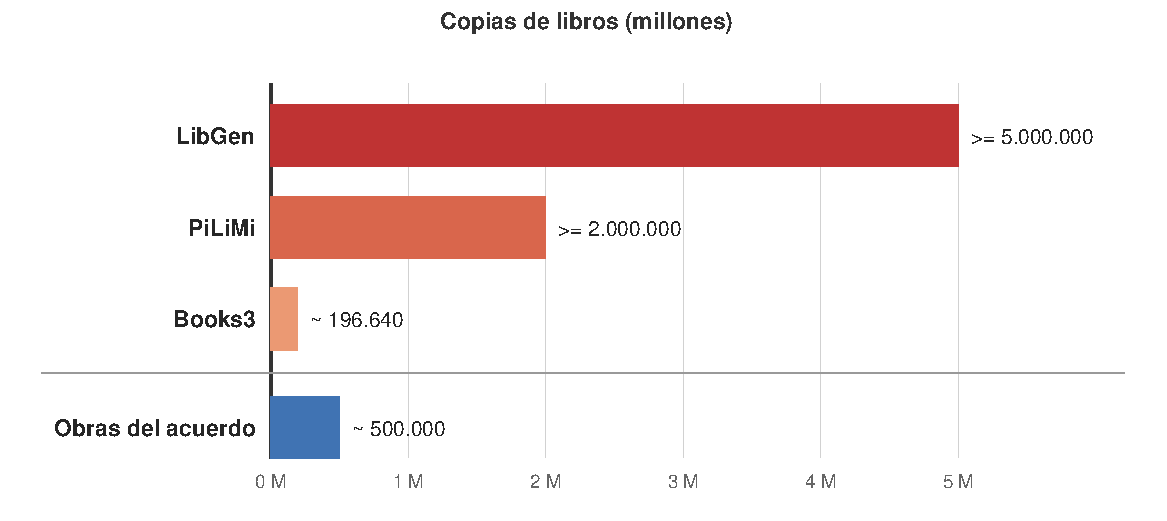
\includegraphics[width=0.85\textwidth]{libros_piratas.pdf}
  \caption[Copias de libros descargadas de fuentes piratas]{Número aproximado de
    copias de libros descargadas de fuentes piratas, según la resolución del caso
    \textit{Bartz}, comparado con las obras cubiertas por el acuerdo final
    (elaboración propia a partir de \cite{bartz2025,npr2025}).}
  \label{fig:piratas}
\end{figure}

Meta se enfrentó a acusaciones parecidas por usar LibGen para entrenar sus modelos
Llama \cite{kadrey2025}. Estos casos demuestran que la carrera por los datos llevó
a varias empresas a \textit{tomar primero y preguntar después}.

% ---------------------------------------------------------------------
\chapter{El caso \textit{Project Panama}}

\section{Comprar, cortar, escanear y tirar}

En febrero de 2024 Anthropic contrató a Tom Turvey, antiguo responsable de
acuerdos de Google Books, para conseguir legalmente \textit{todos los libros del
mundo}. Un documento interno de abril de ese año resumía así el proyecto:
\textit{``Project Panama is our effort to destructively scan all the books in the
world''} \cite{euronews2026}.

El procedimiento, que se resume en la figura~\ref{fig:proceso}, era industrial:

\begin{enumerate}
  \item Se compraban \textbf{libros usados} al por mayor, gastando decenas de
        millones de dólares.
  \item Una guillotina industrial \textbf{cortaba el lomo} para separar las hojas.
  \item Las hojas sueltas pasaban por \textbf{escáneres de alta velocidad}.
  \item El papel restante se enviaba a \textbf{reciclar}.
  \item Las copias digitales se usaban para \textbf{entrenar} a Claude, el modelo de
        la empresa.
\end{enumerate}

\begin{figure}[htbp]
  \centering
  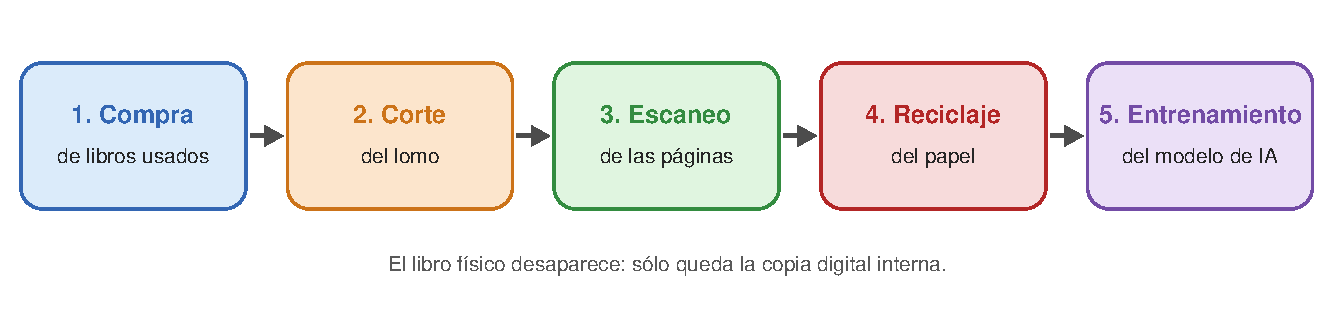
\includegraphics[width=\textwidth]{proceso.pdf}
  \caption[El proceso de escaneo destructivo]{Las cinco fases del escaneo
    destructivo descrito en los documentos judiciales (elaboración propia).}
  \label{fig:proceso}
\end{figure}

Desde el punto de vista económico la lógica es clara: escanear hojas sueltas es
mucho \textbf{más rápido y barato} que escanear un libro encuadernado sin dañarlo,
que es lo que hacía Google Books\footnote{Google Books digitalizó millones de
libros de bibliotecas desde 2004 con escáneres que pasaban las páginas sin
destruir los ejemplares, que volvían a las estanterías.}. El ahorro se paga con la
desaparición del ejemplar físico.

\section{Lo que dijeron los tribunales}

El 23 de junio de 2025 el juez William Alsup dictó una resolución con dos
conclusiones muy distintas \cite{bartz2025}:

\begin{description}
  \item[Escaneo de libros comprados:] es \textit{fair use} (uso legítimo). El
        juez consideró que entrenar una IA es un uso \emph{transformador}, y que
        cambiar el formato de un libro comprado legalmente, destruyendo el
        original, no crea copias adicionales.
  \item[Biblioteca pirata:] \textbf{no} es uso legítimo. Guardar millones de libros
        descargados ilegalmente vulneraba los derechos de los autores.
\end{description}

Ante el riesgo de una indemnización enorme, la empresa llegó a un acuerdo en
septiembre de 2025: \textbf{1\,500 millones de dólares}, unos 3\,000 dólares por
cada una de las cerca de 500\,000 obras afectadas \cite{npr2025}. El acuerdo
recibió la aprobación definitiva en julio de 2026 \cite{latimes2026}. La
tabla~\ref{tab:cronologia} resume las fechas más importantes.

\begin{table}[htbp]
  \centering
  \caption[Cronología del caso]{Cronología del caso \textit{Bartz contra Anthropic}
    y de algunos antecedentes.}
  \label{tab:cronologia}
  \begin{tabular}{@{}lp{0.68\textwidth}@{}}
    \toprule
    \textbf{Fecha} & \textbf{Acontecimiento} \\
    \midrule
    2004           & Google empieza a digitalizar libros sin destruirlos (Google Books). \\
    2021--2022     & Anthropic descarga Books3, LibGen y PiLiMi. \\
    Febrero 2024   & Contratación de Tom Turvey; arranca \textit{Project Panama}. \\
    Agosto 2024    & Los autores A.~Bartz, C.~Graeber y K.~W.~Johnson presentan la demanda. \\
    23 junio 2025  & Resolución del juez Alsup sobre el uso legítimo. \\
    25 junio 2025  & Resolución en \textit{Kadrey contra Meta}. \\
    Septiembre 2025 & Se anuncia el acuerdo de 1\,500 millones de dólares. \\
    2026           & Se hacen públicos los documentos internos de \textit{Project Panama}. \\
    Julio 2026     & Aprobación definitiva del acuerdo. \\
    \bottomrule
  \end{tabular}
\end{table}

% ---------------------------------------------------------------------
\chapter{Análisis: ¿quién gana y quién pierde?}

\section{Comparación de modelos de digitalización}

La tabla~\ref{tab:comparacion} compara las tres formas de conseguir libros que han
aparecido en este trabajo.

\begin{table}[htbp]
  \centering
  \caption[Comparación de formas de obtener libros]{Comparación de tres formas de
    obtener libros para entrenar una IA (valoración propia).}
  \label{tab:comparacion}
  \begin{tabularx}{\textwidth}{@{}lXXX@{}}
    \toprule
    & \textbf{Descarga pirata} & \textbf{Escaneo destructivo} & \textbf{Escaneo no destructivo} \\
    \midrule
    Coste           & Casi nulo        & Medio            & Alto \\
    Velocidad       & Inmediata        & Muy alta         & Lenta \\
    Legalidad (EE.\,UU.) & Ilegal      & Uso legítimo     & Uso legítimo \\
    Pago al autor   & Ninguno          & Ninguno (libros de segunda mano) & Depende del acuerdo \\
    Libro físico    & Se conserva      & \textcolor{red}{\textbf{Se destruye}} & Se conserva \\
    \bottomrule
  \end{tabularx}
\end{table}

\section{Los perdedores}

\begin{itemize}
  \item \textbf{Los autores}: cuando se compra un libro usado, el autor no cobra
        nada, aunque su obra acabe alimentando un producto valorado en miles de
        millones.
  \item \textbf{El patrimonio cultural}: aunque los documentos hablan sobre todo de
        libros usados comprados en grandes lotes, en redes circularon rumores de
        que también se destruían ejemplares raros, algo que verificadores como
        Snopes han analizado \cite{snopes2026}.
  \item \textbf{El público}: las copias digitales no se comparten; se quedan en los
        servidores de la empresa.
\end{itemize}

\section{El contexto legal}

El caso no es único. La Oficina de Derechos de Autor de EE.\,UU. ha estudiado si
entrenar IA con obras protegidas es legal y concluye que la respuesta depende de
cada caso \cite{copyrightoffice2025}. Expertas como Pamela Samuelson llevan años
advirtiendo de que la IA generativa obliga a replantear los derechos de autor
\cite{samuelson2023}.

% ---------------------------------------------------------------------
\chapter{Valoración personal}

\begin{center}
  \Large\textbf{¿Es aceptable destruir libros para ganar dinero?}
\end{center}

\begin{flushleft}
En mi opinión, el caso \textit{Project Panama} muestra muy bien cómo funciona hoy
la industria tecnológica: \textbf{la ley va siempre por detrás}. Lo primero fue
la piratería, y sólo cuando el riesgo legal se hizo evidente se buscó una
alternativa ``legal''. Pero que algo sea legal no significa que sea correcto.
\end{flushleft}

Me parece especialmente preocupante que la destrucción del libro físico se
eligiera por razones de \textit{coste}. Existían técnicas para digitalizar sin
destruir, como demostró Google Books, pero eran más lentas y caras. Por tanto, el
motivo no era técnico, sino \textbf{económico}: maximizar el beneficio y ganar
velocidad en la competencia con otras empresas.

También creo que hay que evitar el alarmismo. Un ejemplar usado de una novela
superventas no es un incunable, y muchos de esos libros probablemente habrían
acabado igualmente en una trituradora. El problema no es tanto cada libro
concreto como el \textit{mensaje} que se transmite: que el libro sólo vale por los
datos que contiene, y que una vez extraídos ya no sirve para nada.

{\footnotesize Paradójicamente, es la misma idea que denunciaba Bradbury: en
\textit{Fahrenheit 451} los libros desaparecían porque la sociedad había dejado de
valorarlos \cite{bradbury1953}.}

\section{Propuestas}

Para terminar, propongo algunas medidas que harían este negocio más justo:

\begin{enumerate}
  \item Exigir \textbf{transparencia} sobre los libros usados para entrenar cada
        modelo.
  \item Crear sistemas de \textbf{licencias} que paguen a los autores, igual que
        las radios pagan por la música que emiten.
  \item Obligar a que la digitalización masiva sea \textbf{no destructiva}, o al
        menos que los ejemplares raros se donen a bibliotecas.
  \item Que las copias digitales sirvan también para \textbf{fines públicos}, por
        ejemplo para la conservación en bibliotecas nacionales.
\end{enumerate}

\begin{flushright}
  \large\textit{Los libros no arden, pero pueden desaparecer igual.}
\end{flushright}

% ---------------------------------------------------------------------
% ---------------------------------------------------------------------
%  Capítulo 6: guion del vídeo final
% ---------------------------------------------------------------------
\chapter{Idea y guion para el vídeo final}

\section{La idea}

El vídeo será una \textbf{recreación de algunas de las quemas de libros más
importantes de la historia}. En cada una se explicará \emph{quién} quemó los
libros, \emph{por qué} lo hizo y \emph{qué conocimiento} se perdió. Al final, la
historia llegará al presente: los libros ya no arden, sino que se cortan, se
escanean y se entregan a una inteligencia artificial.

La idea central es una advertencia:

\begin{center}
  \large\textit{Antes se quemaban libros para que la gente no pensara.\\
  Hoy se los damos a una máquina para no tener que pensar.}
\end{center}

Cuanto más conocimiento y más tareas le entregamos a la IA, más depende la
gente de ella y menos usa su propia cabeza. Un estudio del MIT Media Lab
observó que quienes escribían redacciones con ayuda de ChatGPT mostraban
\textbf{menos actividad cerebral} y recordaban peor lo que habían escrito que
quienes lo hacían sin ayuda \cite{kosmyna2025}\footnote{Es un estudio preliminar
con 54 participantes y otros investigadores han criticado su metodología, así que
en el vídeo se presentará como una señal de alarma, no como una prueba
definitiva.}. El vídeo lleva esa idea al extremo: una IA que, a medida que la
alimentamos, \textbf{nos va apagando}.

\subsection{Datos generales}

\begin{itemize}
  \item \textbf{Duración}: entre 3 y 4 minutos.
  \item \textbf{Formato}: escenas cortas con voz en \textit{off}, imágenes
        recreadas y textos en pantalla.
  \item \textbf{Tono}: serio y algo inquietante, que va de la historia al
        presente.
  \item \textbf{Elemento que se repite}: una \textbf{llama}. En cada escena es
        más pequeña, hasta que al final se convierte en la luz de una pantalla
        que se apaga.
\end{itemize}

\section{Las quemas que se recrearán}

La tabla~\ref{tab:quemas} resume las quemas elegidas y el motivo de cada una.

\begin{table}[htbp]
  \centering
  \caption[Quemas de libros recreadas en el vídeo]{Quemas y destrucciones de
    libros que se recrearán en el vídeo, con sus motivos
    (elaboración propia a partir de \cite{baez2004}).}
  \label{tab:quemas}
  \small
  \begin{tabularx}{\textwidth}{@{}llXX@{}}
    \toprule
    \textbf{Fecha} & \textbf{Lugar} & \textbf{Qué se destruyó} & \textbf{Por qué} \\
    \midrule
    Siglos I a.C.--IV d.C. & Alejandría & La mayor biblioteca de la Antigüedad
      & Guerras, incendios y abandono a lo largo de siglos \\
    213 a.C.  & China   & Libros de historia y filosofía (orden del emperador Qin Shi Huang)
      & \textbf{Control político}: borrar las ideas contrarias al emperador \\
    1258      & Bagdad  & La Casa de la Sabiduría, arrojada al río Tigris
      & \textbf{Conquista}: los mongoles arrasaron la ciudad \\
    1562      & Maní (México) & Códices mayas, quemados por fray Diego de Landa
      & \textbf{Religión}: se consideraban obra del demonio \\
    10 mayo 1933 & Berlín & Unos 20\,000 libros de autores ``no alemanes''
      & \textbf{Ideología}: el nazismo quería eliminar a judíos y opositores \\
    Agosto 1992 & Sarajevo & La Biblioteca Nacional de Bosnia
      & \textbf{Guerra}: destruir la memoria e identidad de un pueblo \\
    2024--2025 & EE.\,UU. & Millones de libros cortados y reciclados (\textit{Project Panama})
      & \textbf{Beneficio económico}: entrenar una IA rápido y barato \\
    \bottomrule
  \end{tabularx}
\end{table}

Todas tienen algo en común: \textbf{quien destruye los libros quiere controlar el
conocimiento}. La diferencia es que en el último caso el conocimiento no
desaparece, sino que pasa a estar \emph{dentro de una máquina privada}.

\section{Guion escena a escena}

\subsection*{Escena 0. Apertura (0:00--0:15)}
\begin{description}
  \item[Imagen:] pantalla negra. Se oye una cerilla que se enciende y aparece una
        pequeña llama.
  \item[Texto:] \textit{``Allí donde se queman libros, se acaba quemando también
        a las personas.'' (H. Heine, 1821)}.
\end{description}

\subsection*{Escena 1. Alejandría (0:15--0:40)}
\begin{description}
  \item[Imagen:] rollos de papiro sobre una mesa, iluminados por velas. Poco a
        poco el humo los cubre.
  \item[Voz en \textit{off}:] ``Aquí estaba todo el saber del mundo antiguo:
        matemáticas, medicina, astronomía. No ardió en una sola noche: se fue
        perdiendo entre guerras y olvido. Nunca sabremos qué había en esos rollos.''
\end{description}

\subsection*{Escena 2. China, 213 a.C. (0:40--1:00)}
\begin{description}
  \item[Imagen:] tablillas de bambú atadas que se echan a una hoguera.
  \item[Voz en \textit{off}:] ``Un emperador quiso que solo existiera una forma
        de pensar: la suya. Ordenó quemar los libros que contaban otra historia.''
\end{description}

\subsection*{Escena 3. Bagdad, 1258 (1:00--1:20)}
\begin{description}
  \item[Imagen:] libros que caen a un río; el agua se vuelve negra.
  \item[Voz en \textit{off}:] ``Se dice que el Tigris bajó negro por la tinta de
        los libros de la Casa de la Sabiduría.''
\end{description}

\subsection*{Escena 4. Maní, 1562 (1:20--1:40)}
\begin{description}
  \item[Imagen:] códices pintados de colores que se doblan con el fuego.
  \item[Voz en \textit{off}:] ``Siglos de historia maya ardieron en una sola
        tarde. Hoy apenas sobreviven cuatro códices.''
\end{description}

\subsection*{Escena 5. Berlín, 1933 (1:40--2:00)}
\begin{description}
  \item[Imagen:] una plaza de noche, siluetas que lanzan libros a una gran hoguera.
  \item[Voz en \textit{off}:] ``Primero quemaron los libros. Después vinieron
        las personas.''
\end{description}

\subsection*{Escena 6. Sarajevo, 1992 (2:00--2:15)}
\begin{description}
  \item[Imagen:] hojas quemadas que caen como si fuera nieve.
  \item[Voz en \textit{off}:] ``Para destruir a un pueblo, primero se destruye
        su memoria.''
\end{description}

\subsection*{Escena 7. El presente: la guillotina (2:15--2:45)}
\begin{description}
  \item[Imagen:] \textbf{cambio brusco}. Luz blanca de fábrica. Una guillotina
        corta el lomo de un libro; las hojas pasan por un escáner y terminan en
        un contenedor de reciclaje.
  \item[Voz en \textit{off}:] ``Hoy los libros ya no arden. Se compran, se cortan,
        se escanean y se tiran. No para que olvidemos, sino para alimentar a una
        máquina. Y para que alguien gane dinero con ello.''
\end{description}

\subsection*{Escena 8. El apagón (2:45--3:30)}
\begin{description}
  \item[Imagen:] una persona frente a una pantalla. Cada vez que le pide algo a
        la IA (``hazme el trabajo'', ``resúmeme el libro'', ``piensa por mí''),
        una luz de la habitación se apaga. Al final solo queda la luz de la
        pantalla sobre su cara.
  \item[Voz en \textit{off}:] ``Le dimos todos los libros. Le dimos nuestras
        preguntas. Y ella nos dio respuestas\ldots{} hasta que dejamos de hacernos
        preguntas.''
  \item[Efecto:] la pantalla se apaga. Negro total.
\end{description}

\subsection*{Escena 9. Cierre (3:30--3:50)}
\begin{description}
  \item[Imagen:] en la oscuridad se enciende una pequeña lámpara. Alguien abre un
        libro de papel y empieza a leer.
  \item[Texto final:] \textcolor{red}{\textbf{Los libros no arden. Pero nosotros
        podemos apagarnos.}}
\end{description}

\section{Notas de producción}

\begin{enumerate}
  \item \textbf{Seguridad}: \emph{no se usará fuego real} sobre libros. Las
        llamas se harán con efectos digitales, vídeos de archivo libres de
        derechos o velas grabadas de cerca. Si se graba alguna llama real, será
        al aire libre, con un adulto, un extintor o un cubo de agua cerca, y
        quemando solo papel de reciclar.
  \item \textbf{No destruir libros de verdad}: sería contradictorio con el mensaje
        del vídeo. Se usarán libros de atrezo, cajas forradas o papel impreso.
  \item \textbf{Material}: móvil para grabar, una lámpara, velas, papel y un
        programa de edición gratuito (por ejemplo, CapCut o DaVinci Resolve).
  \item \textbf{Música y sonidos}: libres de derechos (por ejemplo, la biblioteca
        de audio de YouTube), con crepitar de fuego en las escenas históricas y un
        zumbido eléctrico en las escenas del presente.
  \item \textbf{Rigor}: los textos en pantalla con fechas y datos se revisarán con
        las fuentes de la bibliografía.
\end{enumerate}


% ---------------------------------------------------------------------
\backmatter
\bibliographystyle{apalike}
\bibliography{referencias}

\end{document}
